\documentclass[conference]{IEEEtran}
\IEEEoverridecommandlockouts
% The preceding line is only needed to identify funding in the first footnote. If that is unneeded, please comment it out.
\usepackage[T1]{fontenc}
\usepackage{cite}
\usepackage{mathtools}
\usepackage{stackengine}
\def\delequal{\mathrel{\ensurestackMath{\stackon[1pt]{=}{\scriptstyle\Delta}}}}
\usepackage{amsmath,amssymb,amsfonts}
\usepackage{amsmath,epsfig,cite,amsfonts,amssymb,psfrag,subfig}
\usepackage{graphicx}
\usepackage{textcomp}
\usepackage{xcolor}
\usepackage{algorithm}
\usepackage[noend]{algpseudocode}
\usepackage{amsthm}
\def\BibTeX{{\rm B\kern-.05em{\sc i\kern-.025em b}\kern-.08em
    T\kern-.1667em\lower.7ex\hbox{E}\kern-.125emX}}
\allowdisplaybreaks
\newtheorem{remark}{Remark}
\newtheorem{theorem}{Theorem}
\newtheorem{lemma}{Lemma}
\newtheorem{proposition}{Proposition}
\newtheorem{corollary}{Corollary}
\newcommand{\diag}{\mathop{\mathrm{diag}}}
\DeclareMathOperator{\E}{\mathbb{E}}
\usepackage[margin=0.7in]{geometry}
\setlength{\columnsep}{11mm}
\begin{document}

\title{Questions\vspace{-.1cm}
}
%
%\author{\IEEEauthorblockN{1\textsuperscript{st} Mojdeh Karbalaee Motalleb}
%\IEEEauthorblockA{\textit{Electrical and Computer Engineering} \\
%\textit{Tehran University}\\
%Tehran, Iran \\
%mojdeh.karbalaee@ut.ac.ir}
%\and
%\IEEEauthorblockN{2\textsuperscript{nd} Vahid Shah-Mansouri}
%\IEEEauthorblockA{\textit{Electrical and Computer Engineering} \\
%\textit{Tehran University}\\
%Tehran, Iran \\
%vmansouri@ut.ac.ir}
%\and
%\IEEEauthorblockN{3\textsuperscript{rd} Salar Nouri Naghadeh}
%\IEEEauthorblockA{\textit{Electrical and Computer Engineering} \\
%\textit{Tehran University}\\
%Tehran, Iran \\
%salar.nouri@ut.ac.ir}
%}
  \author{
    \IEEEauthorblockN{Mojdeh Karbalaee Motalleb}
    \IEEEauthorblockA{School of ECE, College of Engineering, University of Tehran, Iran \\
    Email: \{mojdeh.karbalaee\}@ut.ac.ir,
    \vspace{-.2cm}
  }
  }

\maketitle

\begin{abstract}

\end{abstract}
\begin{IEEEkeywords}

\end{IEEEkeywords}
\section{Questions}
\begin{enumerate}
\item \textbf{Why deep Q learning is better than Q learning?}


Deep RL uses a Deep Neural Network to approximate Q(s,a). Non-Deep RL defines Q(s,a) using a tabular function.

Popular Reinforcement Learning algorithms use functions Q(s,a) or V(s) to estimate the Return (sum of discounted rewards). The function can be defined by a tabular mapping of discrete inputs and outputs. However, this is limiting for continuous states or an infinite/large number of states. A more generalized approach is necessary for large number of states.

Function approximation is used for a large state space. A popular function approximation method is Neural Networks. You can make a Deep Neural Network by adding many hidden layers.

Thus, Deep Reinforcement Learning uses Function Approximation, as opposed to tabular functions. Specifically DRL uses Deep Neural Networks to approximate Q or V (or even A).

When the environment gets complicated, the knowledge space can become huge and it no longer becomes feasible to store all (state, action) pairs. If you think about it in raw terms, even a slightly different state is still a distinct state (e.g. different position of the enemy coming through the same corridor). You could use something that can generalize the knowledge instead of storing and looking up every little distinct state.

So, what you can do is create a neural network, that e.g. predicts the reward for an input (state, action) (or pick the best action given a state, however you like to look at it)
So, what you effectively have is a NN that predicts the Q value, based on the input (state, action). This is way more tractable than storing every possible value like we did in the table above.

$Q = neural-network.predict(state, action)$
\begin{figure}%[H]
  \centering
    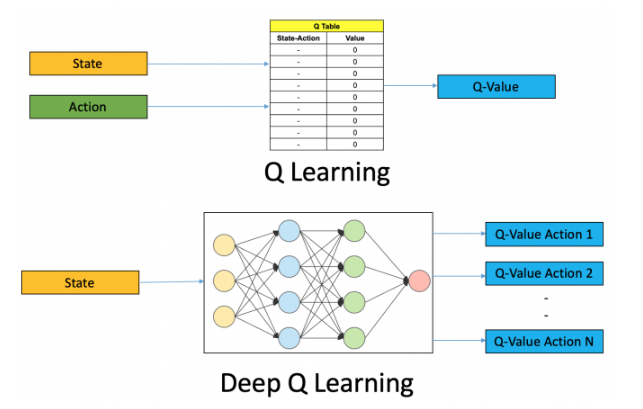
\includegraphics[width=\linewidth]{deepQ}
  \caption{deep Q learning structure \cite{drl}}
  \label{fig:drl}
\end{figure}
\item  \textbf{Find QoS that is required for different applications }
\begin{itemize}
\item \textbf{Bandwidth and throughput}: Bandwidth is the available capacity of connection between two terminals as the most popular term for that is (bps). Throughput slightly differs
from bandwidth as it stands for effective bandwidth that is
provided by network
\item \textbf{Delay or latency:} It specifies the time it takes for a packet
to leave source until reaching the destination. Applications
and network devices can cause delay.
\item \textbf{Jitter (delay variation):} Jitter is an interval between
subsequent packets. It is occurred by network congestion,
route alternation and etc. 
\item \textbf{Loss:} It is amount of packets out of all that are not received
at destination. The success of QOS depends on this factor.
\item \textbf{Reliability:} Some applications are sensitive to packet loss
such as real-time applications. Thus there must be some
mechanism either in application or network to minimize the
packet loss, such as forward error correction (FEC).
\end{itemize}
\begin{figure}%[H]
  \centering
    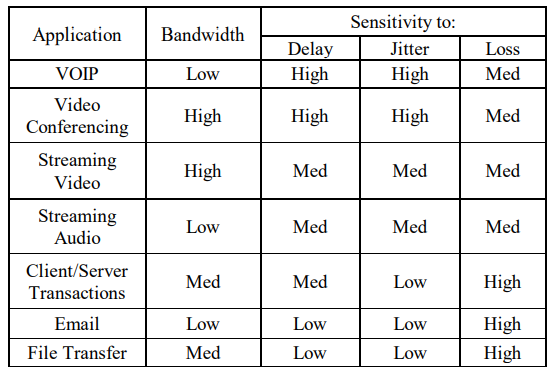
\includegraphics[width=\linewidth]{qos}
  \caption{deep Q learning structure \cite{qos}}
  \label{fig:qos}
\end{figure}
\item \textbf{Where do we use out of order delivery?}

out-of-order delivery is the delivery of data packets in a different order from which they were sent. Out-of-order delivery can be caused by packets following multiple paths through a network, or via parallel processing paths within network equipment that are not designed to ensure that packet ordering is preserved. One of the functions of TCP is to prevent the out-of-order delivery of data, either by reassembling packets into order or forcing retries of out-of-order packets.

Some applications running on your network are sensitive to delay. These applications commonly use the UDP protocol as opposed to the TCP protocol. The key difference between TCP and UDP as it relates to time sensitivity is that TCP will retransmit packets that are lost in transit while UDP does not. For a file transfer from one PC to the next, TCP should be used because if any packets are lost, malformed or arrive out of order, the TCP protocol can retransmit and reorder the packets to recreate the file on the destination PC.
\item \textbf{ What is the best method for online learning?! Game theory vs RL vs DRL vs Deep learning?}

In Reinforcement Learning (RL) it is common to imagine an underlying Markov Decision Process (MDP). Then the goal of RL is to learn a good policy for the MDP, which is often only partially specified. MDPs can have different objectives such as total, average, or discounted reward, where discounted reward is the most common assumption for RL. There are well-studied extensions of MDPs to two-player (i.e., game) settings.

Game theory is quite involved in the context of Multi-agent Reinforcement learning (MARL).

RL: A single agent is trained to solve a Markov decision problem (MDPS). GT: Two agents are trained to solve Games. A multi-agent Reinforcement learning (MARL) can be used to solve for stochastic games.

If you are interested in the single-agent application of RL in deep learning, then you do not need to go for any GT course. For two or more agents you may need to know the game-theoretic techniques.

So a big differences is that mostly RL is a single agent decision and GT is a multiple agent decision.

Then there are minor differences related to the most common uses. RL uses decision through time, GT only equilibria points. RL considers infinite state space, GT considers finite ones. RL is a learning problem (you have to learn the model of the world) while GT is a planning problem (you already know your game matrix). Of course there are exception to all these minor differences.

For instance it is easy to prove that two agents using Q-Learning in a competitive game will converge to the Nash equilibria of a game.
%%
The reinforcement learning techniques enable a single
agent to learn optimal behavior through trial-and-error interactions with its environment. Various RL techniques have been developed which allow an agent to optimize its behavior in a wide range of circumstances. However, when multiple learners simultaneously apply reinforcement learning in a shared environment, the traditional
approaches often fail.
When, in addition to multiple agents, we assume a dynamic environment which
requires multiple sequential decisions, the problem becomes even more complex.
Now agents do not only have to coordinate, they also have to take into account the
current state of their environment. This problem is further complicated by the fact
that agents typically have only limited information about the system.

Game theory is generally defined as the mathematics of conflicts and are being utilized in various fields like economy, psychology, AI, sociology etc. In Game theory w.r.t RL, the policy is the strategy, mapping all possible state of actions, in respect to one of the players of the game.
The types of games in Multi-Agent RL (MARL) are:
Static Games : players are independent and make simultaneous decision

Stage Games : the rules depend on specific stages

Repeated Games : when a game is played in sequence
\begin{figure}%[H]
  \centering
    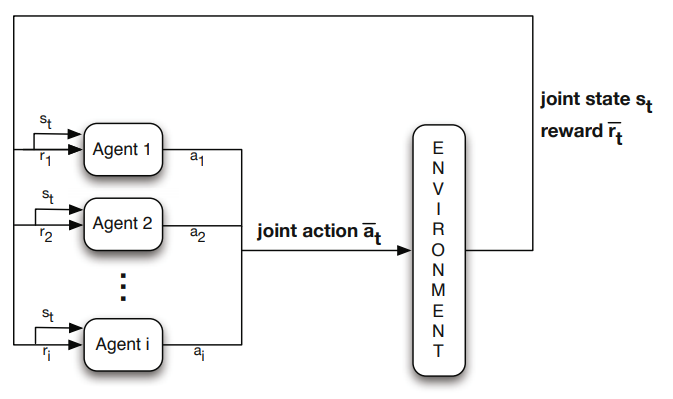
\includegraphics[width=\linewidth]{rlfig}
  \caption{Multiple agents acting in the same environment \cite{rl1}}
  \label{fig:qos}
\end{figure}
%%
An extension of the single agent Markov decision process (MDP) to the multi-agent
case can be defined by Markov Games. In a Markov Game, joint actions are the
result of multiple agents choosing an action independently.
While in normal form games the challenges for reinforcement learners originate
mainly from the interactions between the agents, in Markov games they face the
additional challenge of an environment with state transitions. This means that the
agents typically need to combine coordination methods or equilibrium solvers used
in repeated games with MDP approaches from single-agent RL.
\item  \textbf{Find best delay formula which is the nearest to reality (M/M/1 M/D/1 M/G/1)}
\begin{figure}%[H]
  \centering
    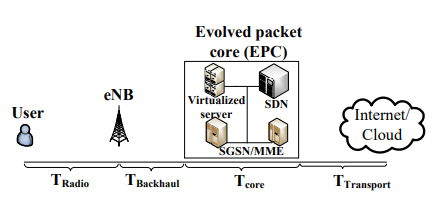
\includegraphics[width=\linewidth]{delay1}
  \caption{ Latency contribution in E2E delay of a packet transmission \cite{delay}}
  \label{fig:delay}
\end{figure}
In the LTE system, the latency can be divided into two
major parts: (1) user plane (U-plane) latency and (2) control
plane (C-plane) latency. The U-plane latency is measured by 
one directional transmit time of a packet to become available
in the IP layer between evolved UMTS terrestrial radio access
network (E-UTRAN) edge/UE and UE/E-UTRAN node.
On the other hand, C-plane latency can be defined as the
transition time of a UE to switch from idle state to active
state. At the idle state, an UE is not connected with radio
resource control (RRC). After the RRC connection is being
setup, the UE switches from idle state into connected state
and then enters into active state after moving into dedicated
mode. Since the application performance is dependent mainly
on the U-plane latency, U-plane is the main focus of interest
for low latency communication.
In the U-plane, the delay of a packet transmission in a
cellular network can be contributed by the RAN, backhaul,
core network, and data center/Internet.
\begin{equation}
T = T_{Radio} + T_{Backhaul} + T_{Core} + T_{Transport}
\end{equation}
\begin{itemize}
\item TRadio

 is the packet transmission time between eNB and
UEs and is mainly due to physical layer communication.
It is contributed by eNBs, UEs and environment. It
consists of time to transmit, processing time at eNB/UE,
retransmissions, and propagation delay. Processing delay at the eNB involves channel coding, rate matching,
scrambling, cyclic redundancy check (CRC) attachment,
precoding, modulation mapper, layer mapper, resource
element mapper, and OFDM signal generation. On the
other hand, uplink processing at UE involves CRC attachment, code block segmentation, code block concatenation, channel coding, rate matching, data and control
multiplexing, and channel interleaver. Propagation delay
depends on obstacles (i.e. building, trees, hills etc.) on
the way of propagation and the total distance traveled by
the RF signal;
\item TBackhaul

 is the time for building connections between
eNB and the core network (i.e. EPC). Generally, the core
network and eNB are connected by copper wires or microwave or optical fibers. In general, microwave involves
lower latency while optic fibers come with comparatively
higher latency. However, spectrum limitation may curb
the capacity of microwave ;
\item TCore

 is the processing time taken by the core network.
It is contributed by various core network entities such
as mobility management entity (MME), serving GPRS
support node (SGSN), and SDN/NFV. The processing
steps of core network includes NAS security, EPS bearer
control, idle state mobility handling, mobility anchoring,
UE IP address allocation, and packet filtering;
\item TTransport

 is the delay to data communication between
the core network and Internet/cloud. Generally, distance
between the core network and the server, bandwidth, and
communication protocol affect this latency
\end{itemize}
\begin{equation}
T_{Radio} = t_{Q} + t_{FA} + t_{tx} + t_{bsp} + t_{mpt}
\end{equation}
\begin{itemize}
\item tQ is the queuing delay which depends on the number of
users that will be multiplexed on same resources;
\item tFA is the delay due to frame alignment which depends on
the frame structure and duplexing modes (i.e., frequency
division duplexing (FDD) and time division duplexing
(TDD));
\item ttx is the time for transmission processing, and payload
transmission which uses at least one TTI depending on
radio channel condition, payload size, available resources,
transmission errors and retransmission;
\item tbsp is the processing delay at the base station;
\item  tmpt is the processing delay of user terminal. Both
the base station and user terminal delay depend on the
capabilities of base station and user terminal (i.e., UE),
respectively.
\end{itemize}
Assume the packet arrival of UEs follows a Poisson process with arrival rate $\lambda$.
It is assumed that there are load balancers in each layer for each slice to divide the incoming traffic to VNFs equally \cite{frdl,luong2018novel,luong2018novel1}.
Suppose the baseband processing of each VNF is depicted as an M/M/1 processing queue.
Each packet is processed by one of the VNFs of a slice. So, the mean delay of  slice in the first and the second layer, modeled as M/M/1 queue, is formulated as follow, respectively
\begin{equation}
\begin{split}
d_{1} &= \frac{1}{\mu_1 - \alpha/{M_{1}}},\\
d_{2} &= \frac{1}{\mu_2 - \alpha/{M_{2}}}.
\end{split}
\end{equation}
where $1/\mu_1$ and $1/\mu_2$ are the mean service time of the first and the second layers respectively.
Besides, $\alpha$ is the  arrival rate which is divided
by load balancer before arriving to the VNFs. The  arrival rate of each VNF in each layer of the slice $s$ is $\alpha/{M_{i}}$ $ i \in \{1,2\}$.
In addition, $d_{tr}$ is the transmission delay on the  wireless link. The arrival data rate of wireless link
 is equal to the arrival data rate of load balancers for each slice \cite{frdl}.
Moreover, it is assumed that the service time of transmission queue for each slice $s$ has
 an exponential distribution with mean $1/(R_{{tot}_s})$ and can be modeled as a M/M/1 queue \cite{frdl,luong2018novel,luong2018novel1,guo2016exploiting}. Therefore,
the mean delay of the transmission layer is
\begin{equation}
 d_{tr} = \frac{1}{R_{{tot}} - \alpha};
\end{equation}
where, $R_{{tot}}$ is the total achievable rate of each slice that is mapped to specific service.
Mean delay of each slice is obtained as below.
\begin{equation}
D_{s} = d_{s_1} + d_{s_2} + d_{{tr}}
\end{equation}
\begin{figure}%[H]
  \centering
    \includegraphics[width=\linewidth]{delay}
  \caption{ delay of a packet \cite{frdl}}
  \label{fig:delay}
\end{figure}
\item \textbf{Assume a system model for the paper}


\textbf{VNF placement after Network Slicing}


Suppose there are $S$ slices Serving $V$ services. Each Service $v\in \{1,2,...,V \} $ consists of $U_v$
 UEs that require certain service. Each slice $s \in \{1,2,...,S \}$  contains VNFs.
There are processing layer in the  system,  represented with a VNF.

Assume we have $M$ VNFs for processing data.
Each VNF  belongs to one or more slices. So, in the $s^{th}$ slice, there are $M_{s}$ VNFs. The VNFs have the computational capacity that is  equal to $\mu$.


Each VNF requires
physical resources that contain memory, storage and CPU.
Let the required resources for VNF $f$ in slice $s$ is represented by a tuple as
\begin{equation}
\bar{\Omega}_{s}^f = \{\Omega_{M,{s}}^f, \Omega_{S,{s}}^f, \Omega_{C,{s}}^f \},
\end{equation}
where $\bar{\Omega}_{s}^f\in \mathbb{C}^{3}$ and $\Omega_{M,{s}}^f, \Omega_{S,{s}}^f, \Omega_{C,{s}}^f$ indicate the amount of required memory, storage, and CPU, respectively.
Moreover, the total amount of required memory, storage and CPU of all VNFs of a slice is defined as
\begin{equation}
\textstyle \bar{\Omega}_{\mathfrak{z},s}^{tot} = \sum_{f=1}^{M_s}\bar{\Omega}_{\mathfrak{z},s}^f \;\; \mathfrak{z} \in \{M, S, C\}.
\end{equation}
Also, there are $D_c$ data centers (DC), serving the VNFs. Each DC contains several servers that supply VNF requirements.
The amount of memory, storage and CPU is denoted by $\tau_{M_{j}}, \tau_{S_{j}}$and $\tau_{C_{j}} $ for the $j^{th}$ DC, respectively
\begin{equation*}
\tau_j = \{\tau_{M_{j}}, \tau_{S_{j}}, \tau_{C_{j}} \},
\end{equation*}
In this system model, the assignment of physical DC resources to VNFs is considered. Let $y_{s,d}$ be a binary variable indicating whether the $d^{th}$ DC is connected to the VNFs of $s^{th}$ slice or not.
Assume the power consumption of baseband processing at each DC $d$ that is connected to VNFs of a slice $s$ is depicted as
$\phi_{s,d}$. So the total power of the system for all active DCs that are connected to slices can be represented as
\begin{equation*}
\textstyle \phi_{tot} = \sum_{s=1}^{S}\sum_{d=1}^{D_c}y_{s,d}\phi_{s,d}.
\end{equation*}
Also, a cost function for the placement of VNFs into DCs is defined as
\begin{equation}\label{eqpsi}
\textstyle  \psi_{tot} = \phi_{tot} - \nu \sum_{d=1}^{D_c}\sum_{v=1}^{V}y_{s,d}a_{v,s}
\end{equation}
where, $\nu$ is a design variable to value between the first term of \eqref{eqpsi} which is the total power consumption of physical resources and the second term that is shown the amount of admitted slices to have physical resources.
\begin{subequations}
\begin{alignat}{4}
\min\limits_{\boldsymbol{y} }   \quad &   \psi_{tot}(\boldsymbol{Y})\\
\text{s. t.} \quad & \textstyle \sum_{d=1}^{D_c}\sum_{v=1}^{V}y_{s,d} \geq 1\times\sum_{v=1}^{V} \forall s, \\
 &\textstyle  \sum_{s=1}^{S} y_{s,d} \bar{\Omega}_{\mathfrak{z},s}^{tot}  \leq   \tau_{\mathfrak{z}_d}  \forall d,, \forall \mathfrak{z}\in \mathcal{E};  \label{eqomega}
\end{alignat}
\end{subequations}
\textbf{RL model}

Here, we need to know agents, states, actions and rewards.
\begin{itemize}
    \item \textbf{Agents} are the services that have slices and each slice have set of VNFs.
    \item \textbf{States}: We have $2^{D_c}$ states that whether each data center is on or off.
    \item \textbf{Actions}: Each action can be defined by connecting set of VNFs of one slice to a DC.
    \item \textbf{Rewards}: the rewards is to minimize the number of using data centers. (minimize power of data centers)
\end{itemize}
%%%
In addition, in each time the deploying a new VNF on a VM needs more power.
\begin{equation*}
\textstyle \phi_{diff} = \sum_{s=1}^{S}\sum_{d=1}^{D_c}[y_{s,d}(t)-y_{s,d}(t-1)]^+\phi_{s,d}^{new}.
\end{equation*}
%%
Also, a cost function for the placement of VNFs into DCs is defined as
\begin{equation}\label{eqpsi}
\textstyle  \psi_{tot} = \phi_{tot} + \phi_{diff}
\end{equation}
where, $\nu$ is a design variable to value between the first term of \eqref{eqpsi} which is the total power consumption of physical resources and the second term that is shown the amount of admitted slices to have physical resources.
\begin{subequations}
\begin{alignat}{4}
\min\limits_{\boldsymbol{y} }   \quad &   \psi_{tot}(\boldsymbol{Y})\\
\text{s. t.} \quad & \textstyle \sum_{d=1}^{D_c}\sum_{v=1}^{V}y_{s,d}(t) \geq 1 \forall s, \\
 &\textstyle  \sum_{s=1}^{S} y_{s,d}(t) \bar{\Omega}_{\mathfrak{z},s}^{tot}  \leq   \tau_{\mathfrak{z}_d}  \forall d,, \forall \mathfrak{z}\in \mathcal{E};  \label{eqomega}
\end{alignat}
\end{subequations}
\item \textbf{Network Slicing}


Suppose there are $S$ slices Serving $V$ services. Each Service $v\in \{1,2,...,V \} $ consists of $U_v$
single-antenna UEs that require certain service. Each slice $s \in \{1,2,...,S \}$ consists of $R_s$ RUs and $K_s$ physical resource blocks (PRBs), one DU and one CU that contains VNFs.
Slices can have shared resources. All RUs in a slice, that are mapped to a service, transmit signals cooperatively to all the UEs in a specific service. Each RU $r \in \{1,2,...,R \}$ is mapped to a DU via an optical fiber link with limited fronthaul capacity.
There are two processing layers one in the DU and one in the CU of ORAN system, each represented with a VNF. The lower layer (i.e., DU) consists of high-PHY, MAC, and RLC, and the upper layer (i.e., CU) consists of RRC, PDCP and SDAP. Assume we have $M_1$ VNFs in the DU layer and $M_2$ VNFs in the CU layer for processing data.
Each VNF in both layers belongs to one or more slices. So, in the $s^{th}$ slice, there are $M_{s,1}$ VNFs in the DU layer and $M_{s,2}$ VNFs in the CU layer. The VNFs in the DU and CU layers have the computational capacity that is  equal to $\mu_1$ and $\mu_2$, respectively.
Also, RUs and PRBs can serve more than one slice.
\subsection{The Achievable Rate}
The achievable data rate for the $i^{th}$ UE in the $v^{th}$ service can be written as
\begin{equation}\label{eq1}
\mathcal{R}_{u(v,i)} = B \log_2({1+ \rho_{u(v,i)}}),
\end{equation}
where $B$ is the bandwidth of system and $\rho_{u(v,i)}$ is the SNR of $i^{th}$ UE in $v^{th}$ service which is obtained from
\begin{equation}\label{eq2}
\rho_{u(v,i)} =  \frac{p_{u(v,i)}\sum_{s=1}^{S}|\bold{h}_{R_s,u(v,i)}^H |^2 a_{v,s}}{BN_0 + I_{u(v,i)}},
\end{equation}
where, $a_{v,s}$ is a binary variable denotes whether the slice $s$ is mapped to service $v$ or not .

\subsection{Mean Delay}
Assume the packet arrival of UEs follows a Poisson process with arrival rate $\lambda_{u(v,i)}$ for the $i^{th}$ UE of the $v^{th}$ service.
Therefore, the mean arrival data rate of UEs mapped to the $s^{th}$ slice in the CU layer is $\alpha_{s_1} = \sum_{v=1}^{V}\sum_{u=2}^{U_v}a_{v,s}\lambda_{u(v,i)}$, where $a_{v,s}$ is a binary variable which indicates whether the $v^{th}$ service is mapped to the $s^{th}$ slice or not.
Furthermore, the mean arrival data rate of the DU layer is approximately equal to the mean arrival data rate of the first layer $\alpha_{s} =\alpha_{s_1} \approx \alpha_{s_2}$ since, by using Burke’s Theorem, the mean arrival data rate of the second layer which is processed in the first layer is still Poisson with rate $\alpha_{s}$.
It is assumed that there are load balancers in each layer for each slice to divide the incoming traffic to VNFs equally \cite{frdl,luong2018novel,luong2018novel1}.
Suppose the baseband processing of each VNF is depicted as an M/M/1 processing queue.
Each packet is processed by one of the VNFs of a slice. So, the mean delay of the $s^{th}$ slice in the first and the second layer, modeled as M/M/1 queue, is formulated as follow, respectively
\begin{equation}
\begin{split}
d_{s_1} &= \frac{1}{\mu_1 - \alpha_{s}/{M_{s,1}}},\\
d_{s_2} &= \frac{1}{\mu_2 - \alpha_{s}/{M_{s,2}}}.
\end{split}
\end{equation}
where $1/\mu_1$ and $1/\mu_2$ are the mean service time of the first and the second layers respectively.
Besides, $\alpha_{s}$ is the  arrival rate which is divided
by load balancer before arriving to the VNFs. The  arrival rate of each VNF in each layer of the slice $s$ is $\alpha_{s}/{M_{s,i}}$ $ i \in \{1,2\}$.
In addition, $d_{s_{tr}}$ is the transmission delay for $s^{th}$ slice on the  wireless link. The arrival data rate of wireless link
 is equal to the arrival data rate of load balancers for each slice \cite{frdl}.
Moreover, it is assumed that the service time of transmission queue for each slice $s$ has
 an exponential distribution with mean $1/(R_{{tot}_s})$ and can be modeled as a M/M/1 queue \cite{frdl,luong2018novel,luong2018novel1,guo2016exploiting}. Therefore,
the mean delay of the transmission layer is
\begin{equation}
 d_{s_{tr}} = \frac{1}{R_{{tot}_s} - \alpha_{s}};
\end{equation}
where, $R_{{tot}_s} =  \sum_{v=1}^{V}\sum_{u=2}^{U_v}a_{v,s}R_{u(v,i)}$ is the total achievable rate of each slice that is mapped to specific service.
Mean delay of each slice is obtained as below.
\begin{equation}
D_{s} = d_{s_1} + d_{s_2} + d_{s_{tr}} \forall s.
\end{equation}
An important criterion to measure the optimality of a system is energy efficiency represented as the sum-rate to sum-power
\begin{equation}
\textstyle \eta(\boldsymbol{P},\boldsymbol{A}) := \frac{\sum\limits_{v=1}^{V} \sum\limits_{k=1}^{{U}_v}\mathcal{R}_{u_{(v,k)}} }{\sum\limits_{s=1}^{S} \sum\limits_{i=1}^{{R}_s}\bar{p}_{r_{(s,i)}}} = \frac{\mathfrak{R}_{tot}(\boldsymbol{P},\boldsymbol{A})}{P_r^{{tot}}(\boldsymbol{P},\boldsymbol{A})},
\end{equation}
where, $P_r^{tot}(\boldsymbol{P},\boldsymbol{A}) = \sum\limits_{s=1}^{S}\sum\limits_{i=1}^{{R}_s}\bar{p}_{r_{(s,i)}}$ is the total power consumption of all RUs in all slices. Also, $\mathfrak{R}_{tot}(\boldsymbol{P},\boldsymbol{A}) = \sum\limits_{v=1}^{V} \sum\limits_{k=1}^{{U}_v}\mathcal{R}_{u_{(v,k)}} $ is the total rates of all UEs applied for all types of services.
The main problem is
\begin{subequations}
\begin{alignat}{4}
\max\limits_{\boldsymbol{P}, \boldsymbol{A} }   \quad &   \eta(\boldsymbol{P},\boldsymbol{A})\\
\text{subject to} \quad  & \bar{p}_{r_{(s,i)}} \leq P_{max} && \quad \forall s, \forall i,   \\
&p_{u_{(v,k)}}  \geq 0  &&\quad \forall v, \forall k, \\
&\mathcal{R}_{u_{(v,k)}} \geq  \mathcal{R}_{u_{(v,k)}}^{min} && \quad \forall v, \forall k, \\
&D_{s} \leq D_{s}^{max}  &&\quad \forall s, \label{cc15} \\
& \textstyle  \sum_{s=1}^{S}a_{v,s} \geq 1 &&\quad \forall s.
\end{alignat}
\label{constraints1}
\end{subequations}
\textbf{RL model}

Here, we need to know agents, states, actions and rewards.
\begin{itemize}
    \item \textbf{Agents}: are the services 
    \item \textbf{States}: set of $A$ and $P$
    \item \textbf{Actions}: Whether service i map to slice j and choose which power.
    \item \textbf{Rewards}: the rewards is to maximize energy efficiency subject to constraints.
\end{itemize}

\end{enumerate}
\bibliographystyle{IEEEtran}
\bibliography{references}
\end{document} 